

%----------------------------------------------------------------------------------------
%	PACKAGES AND DOCUMENT CONFIGURATIONS
%----------------------------------------------------------------------------------------

\documentclass[a4paper,12pt]{article}
\usepackage[margin=0.9in]{geometry}
\renewcommand{\baselinestretch}{1.2}
\usepackage{siunitx} % Provides the \SI{}{} and \si{} command for typesetting SI units
\usepackage{graphicx} % Required for the inclusion of images
\usepackage{subfigure}
\usepackage{multirow}
\usepackage{amsmath} % Required for some math elements 
\usepackage{indentfirst}
%\usepackage{times} % Uncomment to use the Times New Roman font
\usepackage{appendix}
\usepackage{verbatim}


%----------------------------------------------------------------------------------------
%	DOCUMENT INFORMATION
%----------------------------------------------------------------------------------------
\title{ \rule{\textwidth}{0.3mm} \\YALE UNIVERSITY \\ COMPUTATIONAL METHODS FOR INFORMATICS \\ (BIS634) \\ \rule{\textwidth}{0.3mm} \\ [30 mm]  \Large{Final Project Report} \\[5 mm]  Stroke Prediction and Analysis \\[15 mm]} % Title
\author{Cao Zhiyuan} % Author name
\date{\today} % Date for the report

\begin{document}
\scshape

\maketitle % Insert the title, author and date

\begin{center}
\begin{tabular}{l l}
\\[16 mm]
Partners:  \\
Name: Cao Zhiyuan & NedID: zc347 \\
\end{tabular}
\end{center}
\thispagestyle{empty}


\newpage


\small\tableofcontents
\thispagestyle{empty}


\newpage

%----------------------------------------------------------------------------------------
%	SECTION 1
%----------------------------------------------------------------------------------------

\setcounter{page}{1}
\section{\textsc{Introduction}}
\upshape
A stroke is a medical condition in which the blood supply to a part of the brain is disrupted, leading to brain cell death and possible long-term disability or death. Stroke is a leading cause of death and disability worldwide, with high rates of morbidity and mortality. It is worth paying attention to stroke because it can have a significant impact on an individual's quality of life and can also have a significant economic burden on society.

In order to better understand and ultimately prevent or treat stroke, it is important to analyze data on stroke incidents and outcomes. Choosing a dataset for stroke analysis can help researchers and healthcare professionals gain insights into the risk factors, causes, and consequences of stroke, as well as identify potential interventions or treatments that may be effective in reducing the incidence and severity of stroke. By analyzing data on stroke, we can improve our understanding of this important public health issue and work towards finding solutions to reduce the burden of stroke on individuals and society.

\begin{figure}[h] 
    \centering
    
\includegraphics[width=1\textwidth]{home_p1} 
    \caption{Webpage for Homepage} 
\end{figure}

%----------------------------------------------------------------------------------------
%	SECTION 2
%----------------------------------------------------------------------------------------

\section{\textsc{Dataset Description}}
\subsection{\textsc{About the Dataset}}
The dataset named "Stroke Prediction" is an open source dataset from Kaggle. It is under the healthcare-dataset-stroke-data.csv file. The data contains 5110 rows and 12 features in total. The metadata of this datset is also available on Kaggle.

Dataset citation: FEDESORIANO. Stroke Prediction Dataset. Retrieved December 17, 2022 from https://www.kaggle.com/datasets/fedesoriano/stroke-prediction-dataset?resource=download.
\subsection{\textsc{Features}}
\begin{itemize}
\item id: unique identifier of a patient
\item gender: "Male", "Female" or "Other"
\item age: age of the patient
\item hypertension: 0 if the patient doesn't have hypertension, 1 if the patient has hypertension
\item heart\textunderscore disease: 0 if the patient doesn't have any heart diseases, 1 if the patient has a heart disease
\item ever\textunderscore married: "No" or "Yes"
\item work\textunderscore type: "children", "Govt\textunderscore jov", "Never\textunderscore worked", "Private" or "Self-employed"
\item Residence\textunderscore type: "Rural" or "Urban"
\item avg\textunderscore glucose\textunderscore level: average glucose level in blood
\item smoking\textunderscore status: "formerly smoked", "never smoked", "smokes" or "Unknown"*
\item stroke: 1 if the patient had a stroke or 0 if not
\end{itemize}
\subsection{\textsc{Dateframe}}
\begin{figure}[h] 
    \centering
    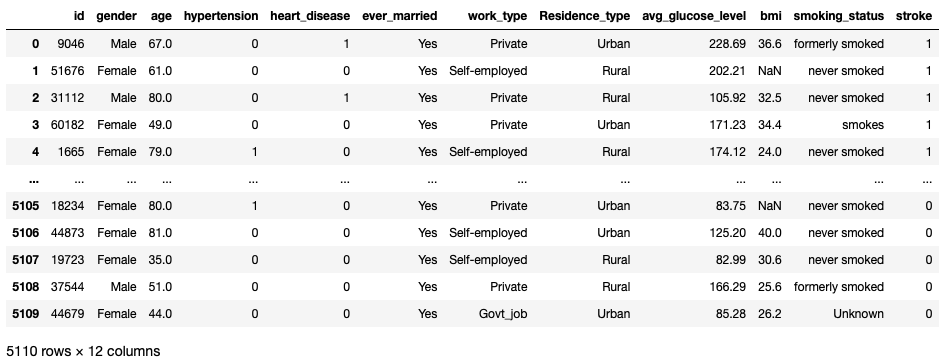
\includegraphics[width=1\textwidth]{p1} 
    \caption{Stroke Prediction Dataframe} 
\end{figure}
\subsection{\textsc{Data Preprocessing}}
\begin{itemize}
\item Data Cleaning: I drop all the rows with missing value 'nan'. After doing so, the dataset contains 4909 rows. Except these missing values, the dataset is very clean and does not need further cleaning: The author has already performed necessary data cleaning.
\item Data processing: I transform all the categorical data into dummy ones to enable machine learning models to process them.
\end{itemize}
\subsection{\textsc{Data FAIRness}}
\begin{itemize}
\item Findability: The stroke dataset is properly documented and has clear and accurate metadata. Hence, it is easy for others to discover and locate it.
\item Accessibility: The stroke dataset is available in a format that is easy to use and that there are no barriers to accessing the data: It is totally free and liscensed by the author. Thus, the dataset can be easily accessible to those who need it.
\item Interoperability: Using standardized formats and providing clear documentation about the data's structure and content, the dataset has a good interoperability, since it can be easily integrated with other datasets or tools.
\item Reusability: The dataset provides clear documentation about the data's provenance, as well as any relevant ethical or legal considerations. Hence the dataset can be easily reused for multiple purposes.
\end{itemize}
\subsection{\textsc{Website Interface}}
\begin{figure}[h] 
    \centering
    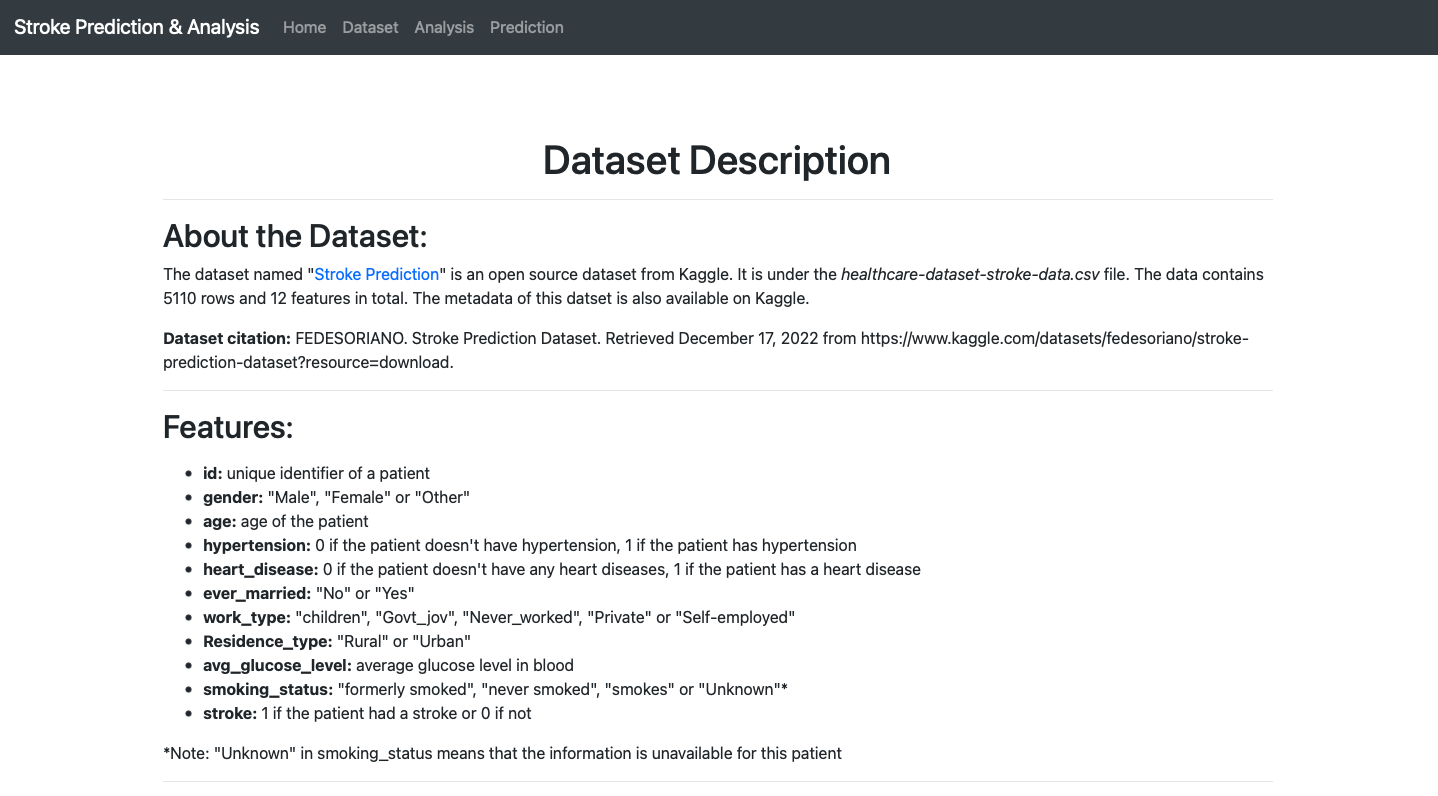
\includegraphics[width=1\textwidth]{home_p6} 
    \caption{Webpage for Dataset Description} 
\end{figure}
\newpage

%----------------------------------------------------------------------------------------
%	SECTION 3
%----------------------------------------------------------------------------------------
\section{\textsc{Exploratory Analysis}}
\subsection{\textsc{Summary Statistics}}
\subsubsection{\textsc{Statistical Analysis}}
\begin{figure}[h] 
    \centering
    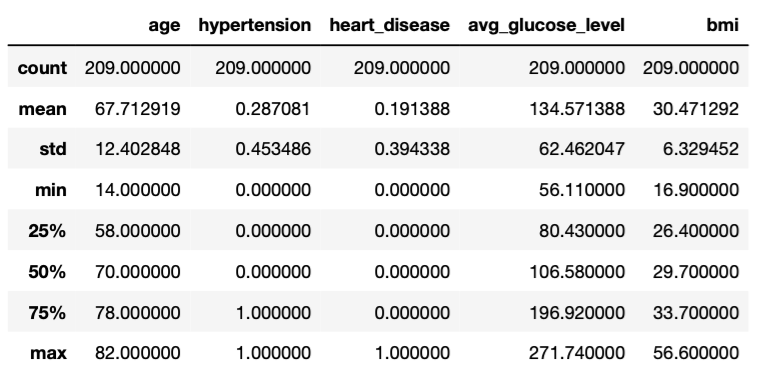
\includegraphics[width=.5\textwidth]{stat_p1} 
    \caption{Summary statistics for patients with stroke} 
\end{figure}
\begin{figure}[h] 
    \centering
    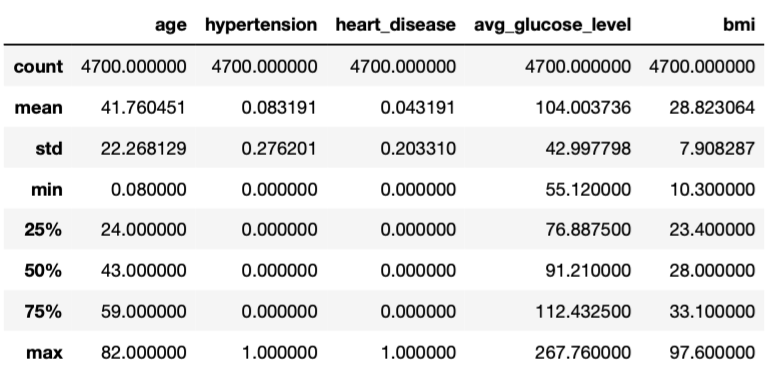
\includegraphics[width=.5\textwidth]{stat_p2} 
    \caption{Summary statistics for patients without stroke} 
\end{figure}
From the statistics, it is clear that:
\begin{itemize}
\item The mean age for people with stroke is much higher than those without stroke. Patients with stroke tends to be 26 years elder than the healthy on average.
\item Patients with stroke have higher probability to have hypertension than healthy people.
\item Patients with stroke have slightly higher probability to have heart disease than healthy people.
\item Patients with stroke tends to have a higher average glucose level than healthy people.
\end{itemize}
\par In conclusion, elder people with other chronic diseases have a higher possiblility to have stroke.

\subsubsection{\textsc{Data Distribution and Outliers Analysis}}
\begin{figure}[h] 
    \centering
    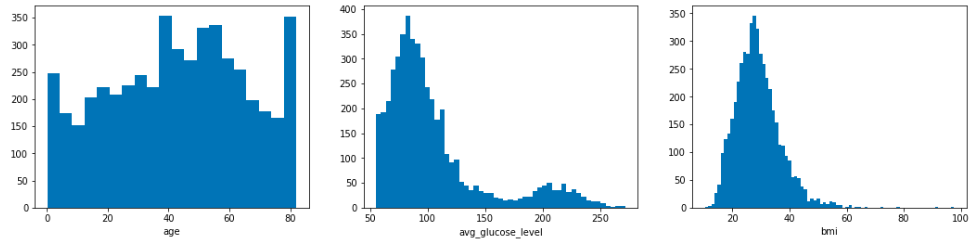
\includegraphics[width=.7\textwidth]{stat_p4} 
    \caption{Histogram for features} 
\end{figure}
\begin{figure}[h] 
    \centering
    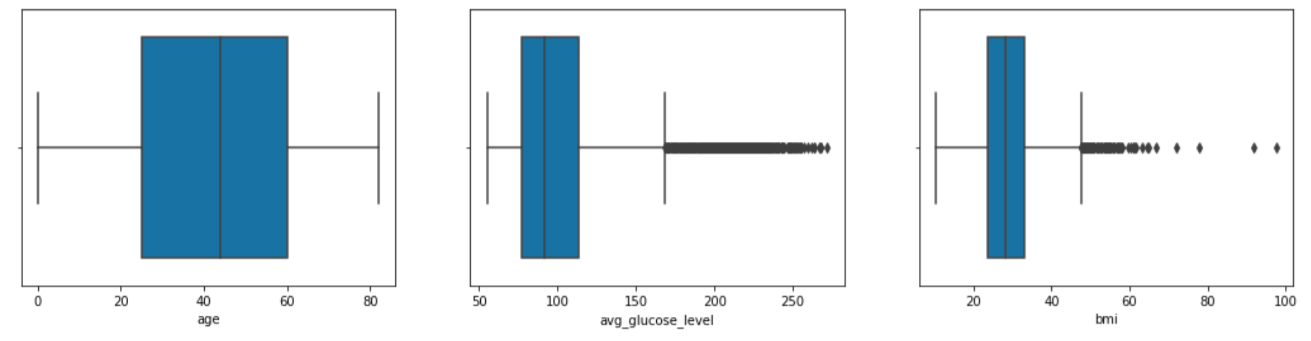
\includegraphics[width=.7\textwidth]{stat_p3} 
    \caption{Bar plot for features} 
\end{figure}
In our dataset, there are three numberic features. The above figure are histogram and barplot, which shows the distribution of these data. From the figure:
\begin{itemize}
\item There is no outlier for age.
\item There are a lot of outliers for avg glucose level and bmi. All the outlier are high values.
\end{itemize}

\newpage
\subsubsection{\textsc{Website Interface}}
\begin{figure}[h] 
    \centering
    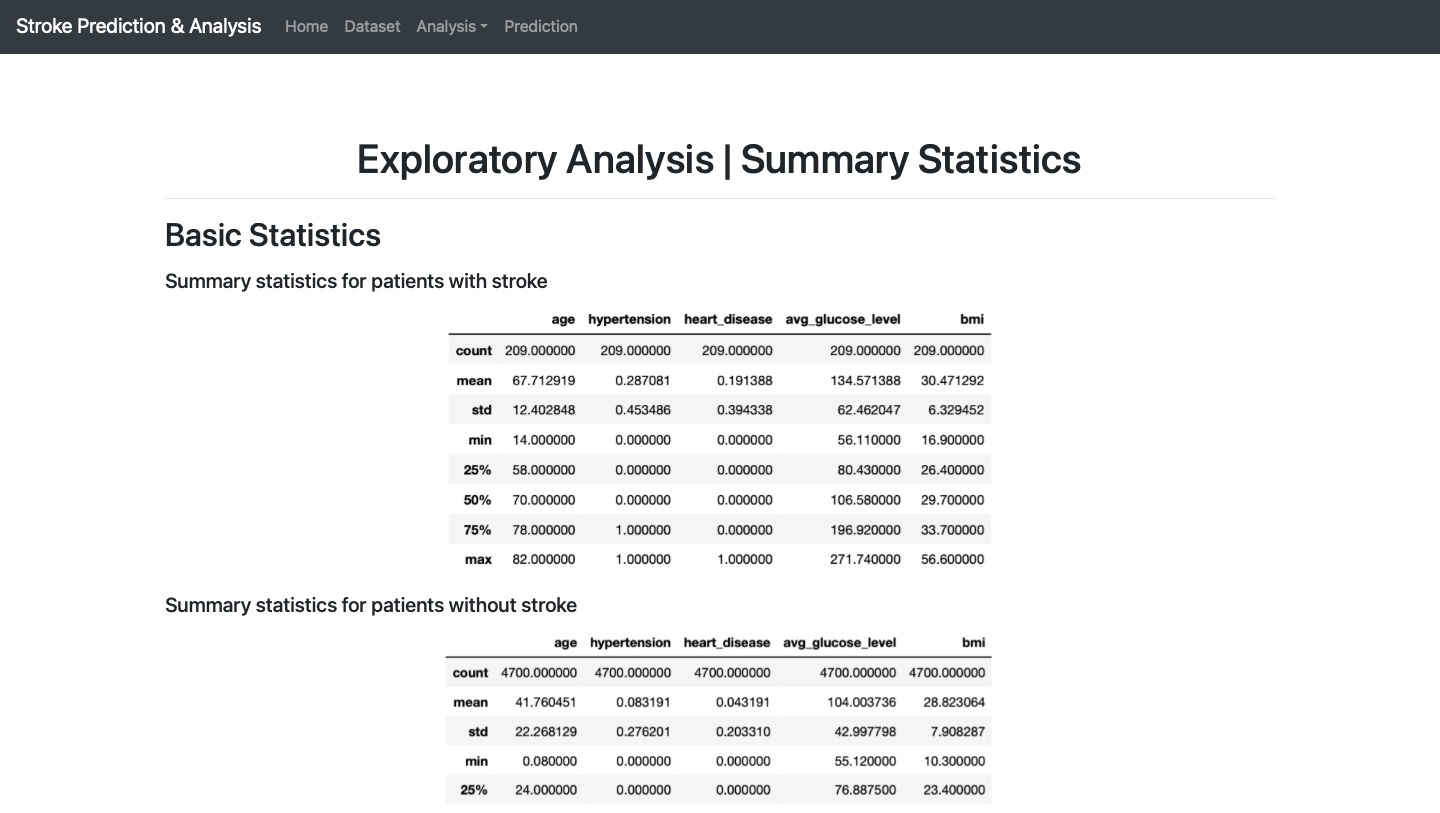
\includegraphics[width=1\textwidth]{ss} 
    \caption{Webpage for Summary Statistics} 
\end{figure}


\newpage


\subsection{\textsc{Univariate Analysis}}
\subsubsection{\textsc{Analysis Questions}}
\begin{itemize}
\item Which age/gender has the highest probability to have stroke?
\item How avg glucose level and bmi related to stroke?
\end{itemize}
\subsubsection{\textsc{Age Distribution}}
\begin{figure}[h] 
    \centering
    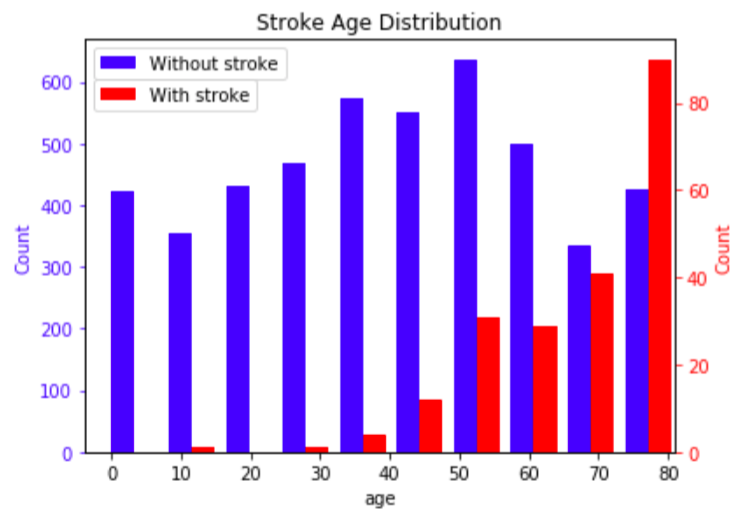
\includegraphics[width=.7\textwidth]{uni_p6} 
    \caption{Histogram for age distribution} 
\end{figure}
The larger the age is, the more possible a person have stroke.
\subsubsection{\textsc{Gender Distribution}}
\begin{figure}[h] 
    \centering
    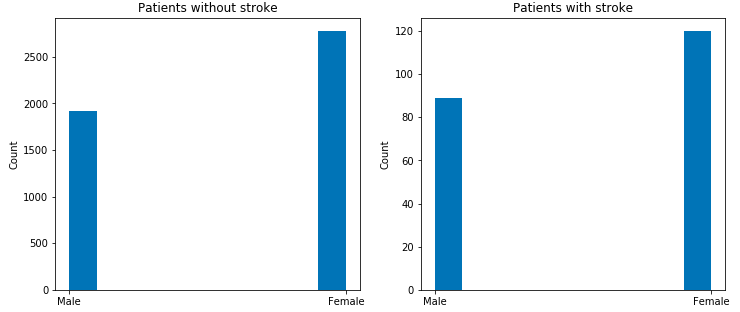
\includegraphics[width=.7\textwidth]{uni_p3} 
    \caption{Histogram for gender distribution} 
\end{figure}
The dataset contains more female patients than male ones. By comparing the proportion of gender within different groups, it can be concluded that there is no strong relationship between gender and stroke.
\subsubsection{\textsc{Glucose Distribution}}
\begin{figure}[h] 
    \centering
    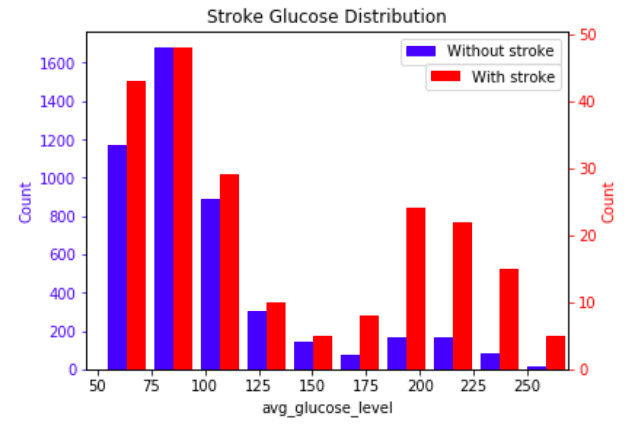
\includegraphics[width=.7\textwidth]{uni_p4} 
    \caption{Histogram for glucose distribution} 
\end{figure}
From the histogram, a higher glucose level do suggest a higher probability  to have stroke. However, for patients with regular average glucose levels, the probability of having stroke won't decrease.

\subsubsection{\textsc{BMI Distribution}}
\begin{figure}[h] 
    \centering
    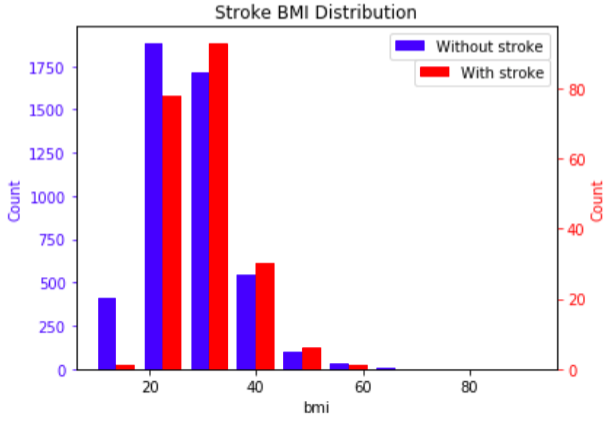
\includegraphics[width=.7\textwidth]{uni_p5} 
    \caption{Histogram for BMI distribution} 
\end{figure}
The histogram suggests that stroke patients tend to have a higher bmi. There exists a weak correlation between bmi and stroke.

\subsubsection{\textsc{Website Interface}}
\begin{figure}[h] 
    \centering
    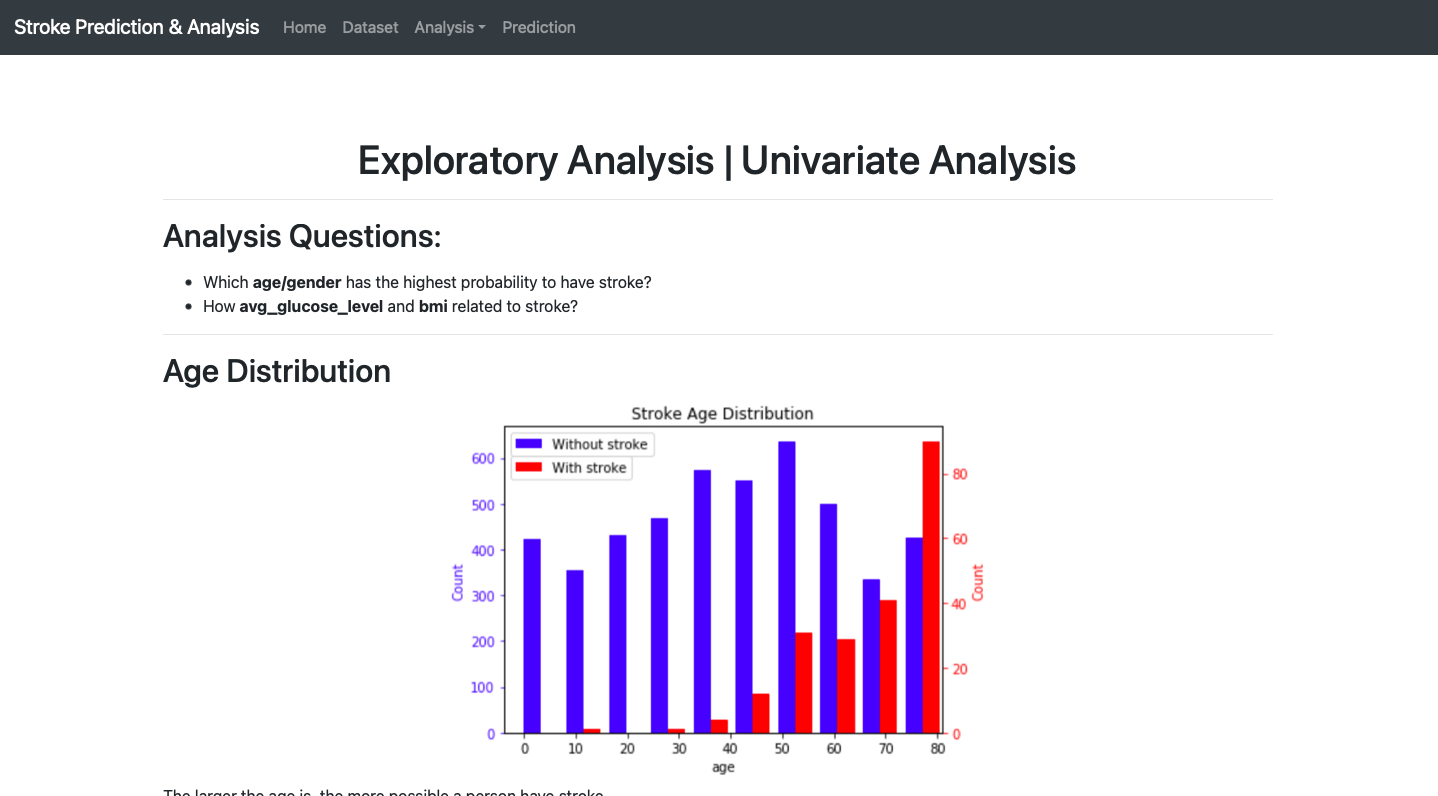
\includegraphics[width=1\textwidth]{home_p7} 
    \caption{Webpage for Summary Statistics} 
\end{figure}

\newpage
\subsection{\textsc{Bivariate Analysis}}
\begin{figure}[h] 
    \centering
    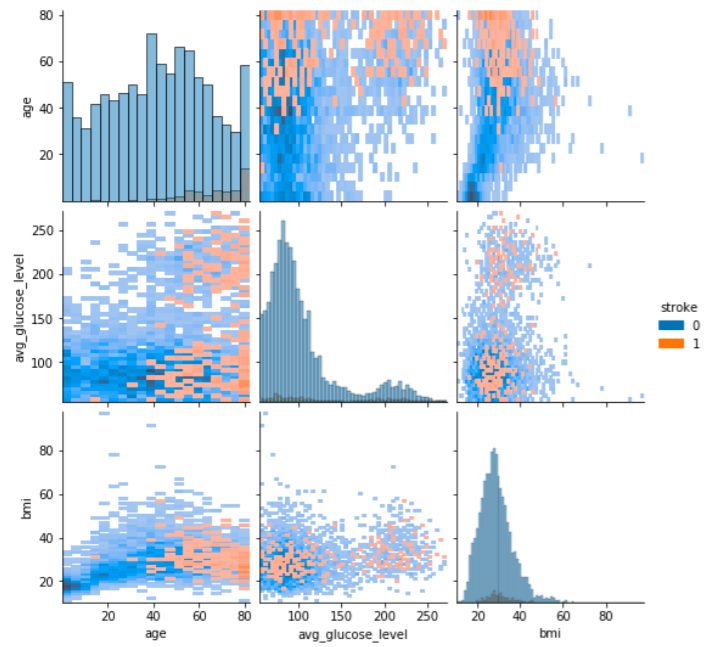
\includegraphics[width=.8\textwidth]{biv_p2} 
    \caption{Summary plot for features} 
\end{figure}
The above figure is the pairplot of three numeric features: age, avg glucose level and bmi. 
Patients with higher age are more likely to have stroke. 
A higher average glucose level and a larger bmi are more likely to result in stroke.

\newpage
\subsubsection{\textsc{Website Interface}}
\begin{figure}[h] 
    \centering
    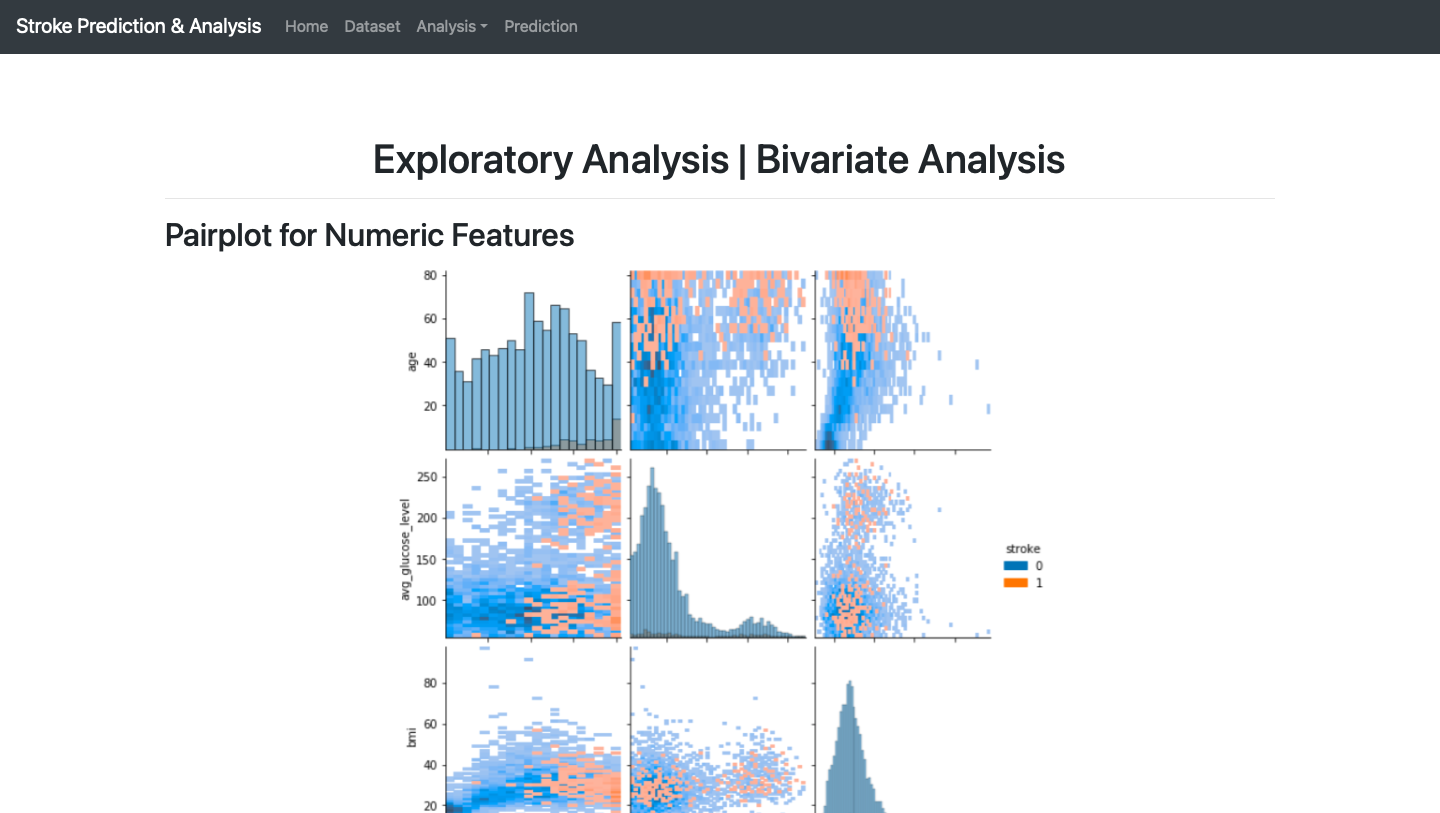
\includegraphics[width=1\textwidth]{ba} 
    \caption{Webpage for Bivariate Analysis} 
\end{figure}

\subsection{\textsc{Feature Correlation}}
\begin{figure}[h] 
    \centering
    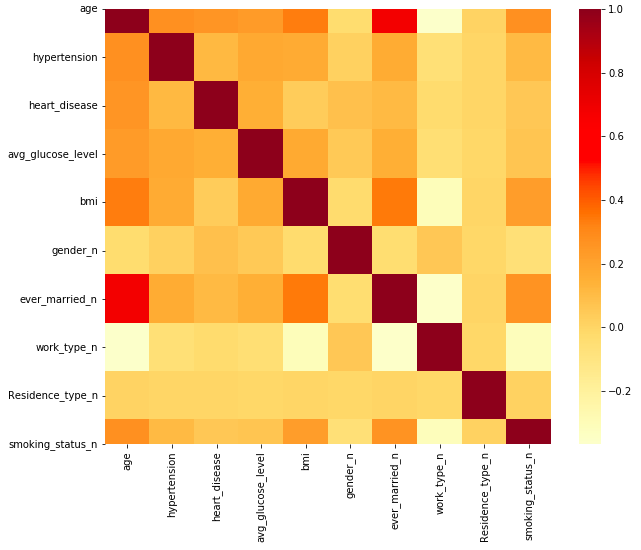
\includegraphics[width=.5\textwidth]{corr_p1} 
    \caption{Correlation matrix for all features} 
\end{figure}

First, I transform all the categorical features into numeric ones.

Then I plot the correlation matrix of the 10 features. The heatmap shows the Pearson correlation coefficients between the features in my dataset. The relationships between the features can then be identified and how they may affect the target variable be understood.

The Pearson correlation coefficient is a measure of the linear relationship between two variables. It ranges from -1 to 1, where -1 indicates a strong negative relationship, 0 indicates no relationship, and 1 indicates a strong positive relationship. A correlation matrix can help identify which features are highly correlated with each other and which are not.

If two features are highly correlated, it may be beneficial to remove one of them from the model to avoid overfitting and improve the model's performance. From the result, it is shown that there does not exist two features that are highly correlated. Thus I keep all the 10 features to train the models.

\subsubsection{\textsc{Any surprise}}
The feature correlation are small, so I keep all these features.


\subsubsection{\textsc{Website Interface}}
\begin{figure}[h] 
    \centering
    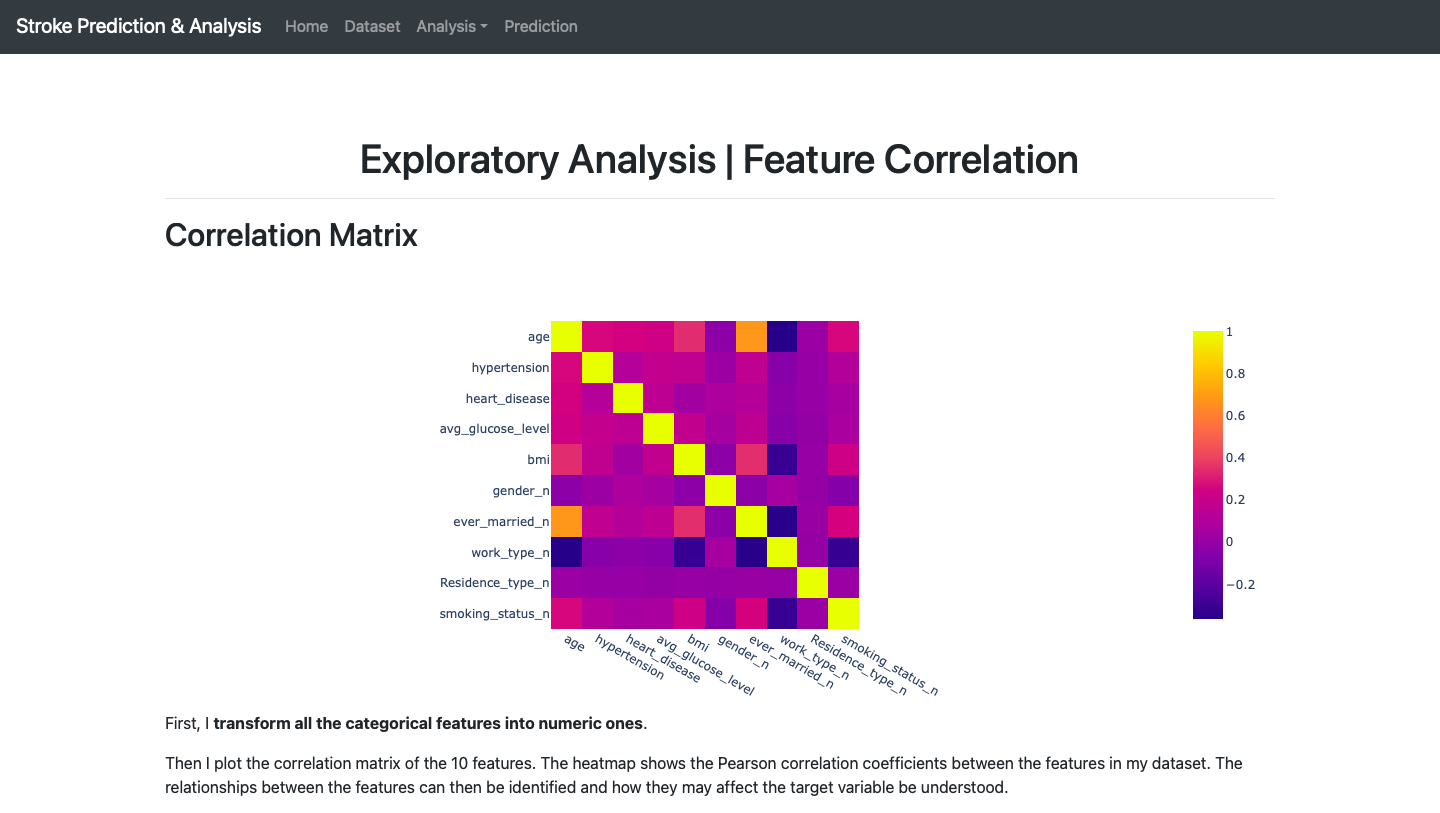
\includegraphics[width=1\textwidth]{fc} 
    \caption{Webpage for Feature Correlation} 
\end{figure}


%----------------------------------------------------------------------------------------
%	SECTION 4
%----------------------------------------------------------------------------------------

\section{\textsc{Prediction}}
I choose two model for prediction. One is XGBoost.
\subsection{\textsc{Performance of XGBoost}}
XGBoost (eXtreme Gradient Boosting) is a popular and efficient open-source implementation of the gradient boosting algorithm for machine learning.

Gradient boosting is a machine learning technique for regression and classification problems, which produces a prediction model in the form of an ensemble of weak prediction models, typically decision trees. The main idea behind gradient boosting is to train weak models sequentially, each trying to correct the mistakes of the previous model.

Overall, XGBoost is a powerful and flexible tool for implementing gradient boosting and is well-suited for a wide range of machine learning tasks.

\begin{figure}[h] 
    \centering
    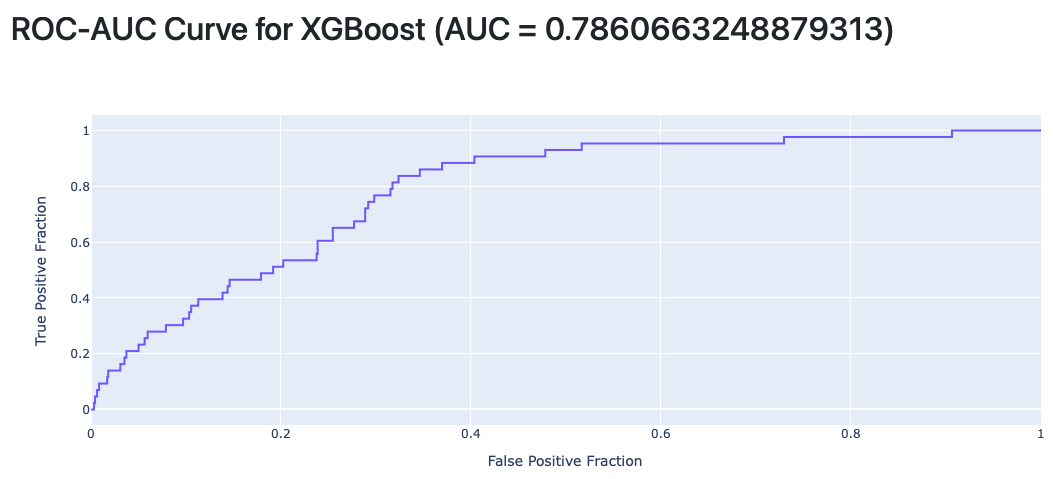
\includegraphics[width=1\textwidth]{bst_p1} 
\end{figure}

\begin{figure}[h] 
    \centering
    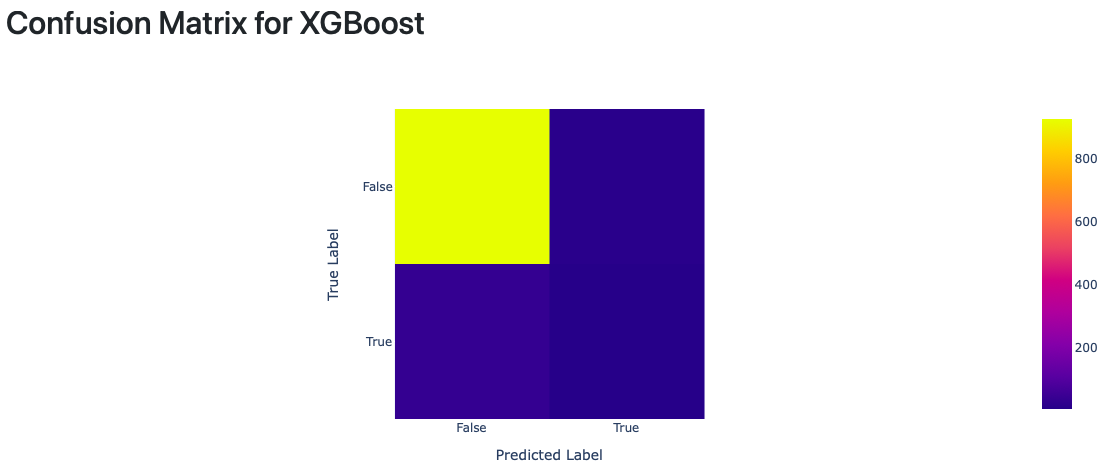
\includegraphics[width=1\textwidth]{bst_p2} 
\end{figure}

\subsection{\textsc{Performance of Random Forest}}
Random Forest is a popular and powerful ensemble machine learning algorithm that is used for classification and regression tasks.

Random Forest is a flexible and easy-to-use algorithm that can handle a large number of input features and can deal with missing values and categorical variables automatically. It is also relatively resistant to overfitting, due to the way it combines multiple decision trees.

Overall, random forest is a widely used and robust machine learning algorithm that is well-suited for many applications.

\begin{figure}[h] 
    \centering
    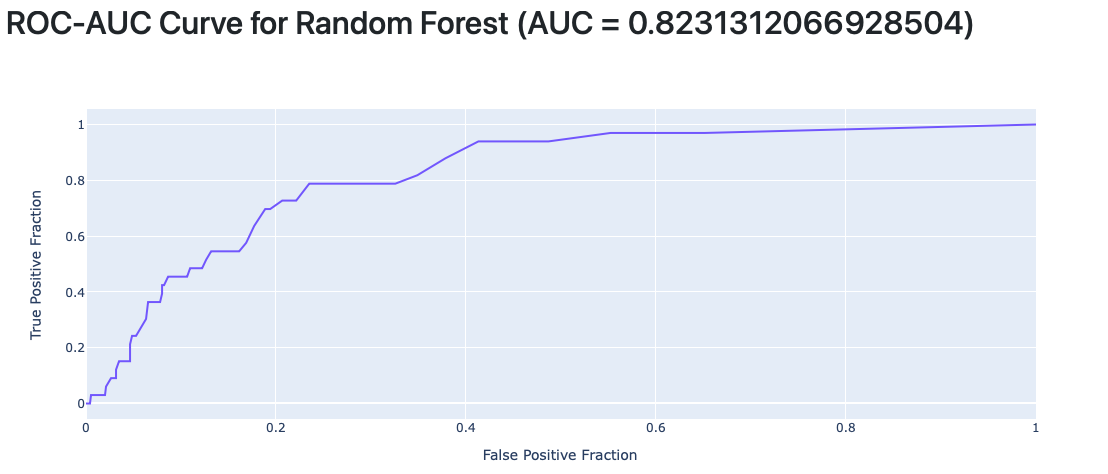
\includegraphics[width=1\textwidth]{rfst_p1} 
\end{figure}

\begin{figure}[h] 
    \centering
    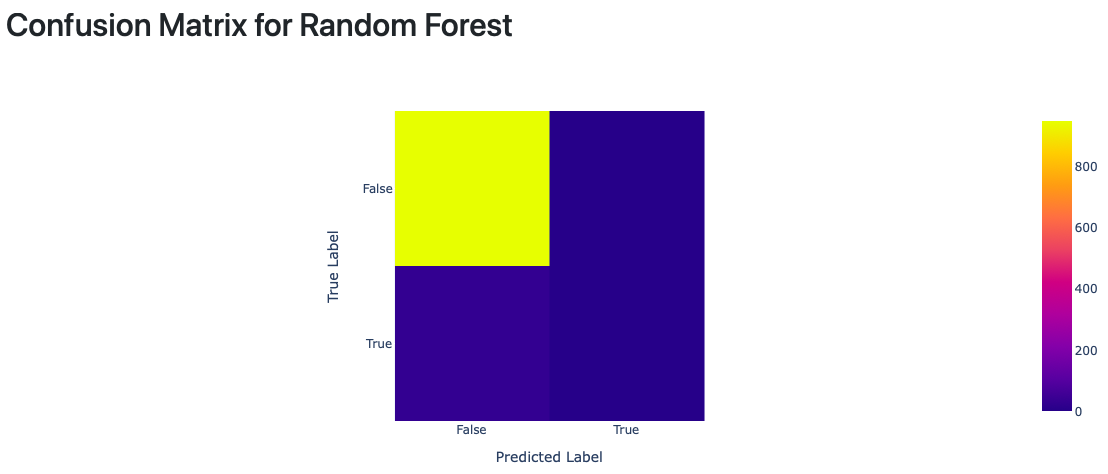
\includegraphics[width=1\textwidth]{rfst_p2} 
\end{figure}
~
\newpage
\subsubsection{\textsc{Website Interface}}
\begin{figure}[h] 
    \centering
    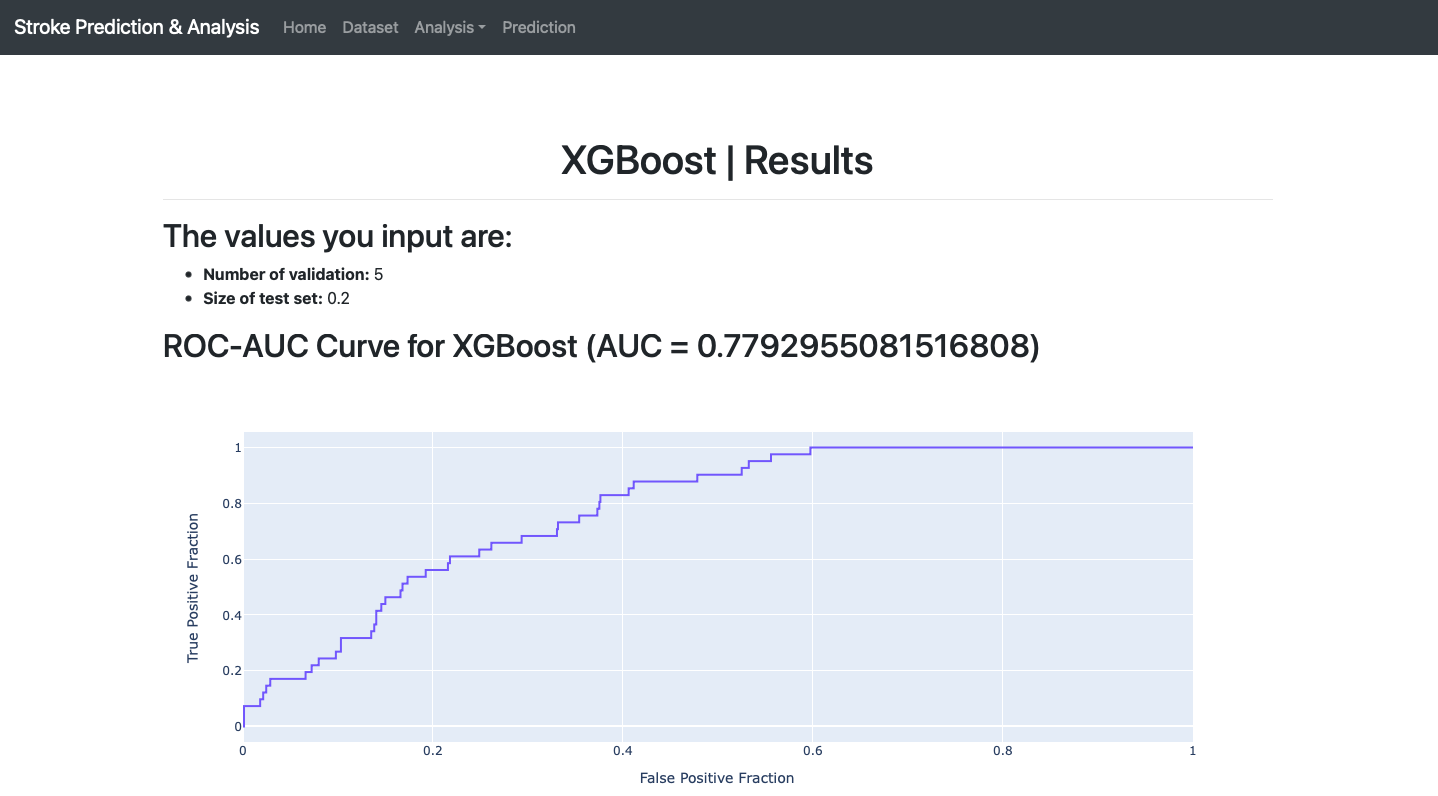
\includegraphics[width=1\textwidth]{home_p8} 
    \caption{Webpage for Feature Correlation} 
\end{figure}

%----------------------------------------------------------------------------------------
%	SECTION 5
%----------------------------------------------------------------------------------------
\section{\textsc{Findings and Limitations}}
The findings of my final project includes:
\begin{itemize}
\item Patients with higher age are more likely to have stroke.
\item A higher glucose level do suggest a higher probability to have stroke.
\item Stroke patients tend to have a higher bmi.
\item Both XGboost and Random Forest have satisfactory performance for predicting stroke. Among them, Random Forest is better and have higher AUC.
\end{itemize}

The limitations of my final project includes:
\begin{itemize}
\item Too many healthy patients compared with the number of stroke patients, making the false positive rate high.
\item The dataset contains 5110 patients. The size of dataset may not be large enough.
\end{itemize}

%----------------------------------------------------------------------------------------
%	SECTION 5.2
%----------------------------------------------------------------------------------------

\section{\textsc{Conclusion}}
In conclusion, in this final project, I analyze stroke prediction dataset and use XGBoost and Random Forest to make prediction. The results are satisfactory. I also made a website which have all the information on it. 

%----------------------------------------------------------------------------------------
%	SECTION 6
%----------------------------------------------------------------------------------------


%----------------------------------------------------------------------------------------
%	BIBLIOGRAPHY
%----------------------------------------------------------------------------------------

%\begin{thebibliography}{9}

%\end{thebibliography}



%----------------------------------------------------------------------------------------


\end{document}
